\newpage %CV


\pagestyle{empty}


%\begin{table}[H]
	%\centering
	%	\caption{}
	%\label{tab:my-table}
	%\resizebox{\textwidth}{!}{%
		%\begin{tabular}{lp{0.05cm}p{7.5cm}}
			%\centering
			%\raisebox{-\totalheight}{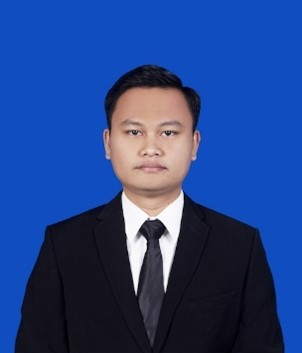
\includegraphics[scale=0.5]{foto_cv_guntur.jpg}} & & %\vspace{0.05cm}\LARGE \textbf{RIWAYAT HIDUP}\\
%			
%		\end{tabular}
%	}
%\end{table}

\centering \large \textbf{RIWAYAT HIDUP}\\
\hspace{1,2cm}
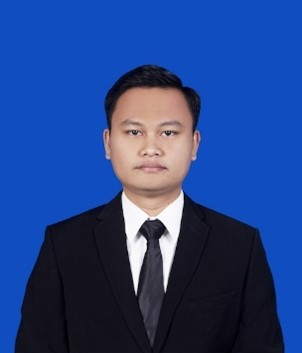
\includegraphics[width=0.2\textwidth, left]{foto_cv_guntur.jpg}

\vspace{1cm}
\noindent \textbf{IDENTITAS DIRI}
\vspace{0.2cm}


\begin{table}[H]
	%	\caption{}
	\label{tab:my-table}
	%	\resizebox{\textwidth}{!}
\end{table}


%\vspace{8cm}
\noindent \textbf{PENDIDIKAN FORMAL}
\vspace{0.2cm}

% Please add the following required packages to your document preamble:
% \usepackage{graphicx}
\begin{table}[H]
		\centering
	%	\caption{}
	\label{tab:my-table}
	%	\resizebox{\textwidth}{!}{%
	\begin{longtable}{|c|l|p{5cm}|}
		\hline
		\textbf{Tahun} & \multicolumn{1}{c|}{\textbf{Pendidikan}} & \multicolumn{1}{c|}{\textbf{Institusi}} \\ \hline
		2009 & S1 Teknik Informatika & Universitas Gunadarma         \\ \hline
		2013 & S2 Manajemen  Sistem Informasi & Universitas Gunadarma  \\ \hline
		2019 & S3 Teknologi Informasi & Universitas Gunadarma \\ \hline
	\end{longtable}%
	%	}
		\centering	
\end{table}

%\newpage
%\vspace{0.5cm}
\newpage
\noindent \textbf{PENGALAMAN KERJA}
\vspace{0.2cm}


% Please add the following required packages to your document preamble:
% \usepackage{graphicx}
\begin{table}[H]
		\centering
	%	\caption{}
	%	\label{tab:my-table}
	%	\resizebox{\textwidth}{!}{%
	\begin{tabular}{|l|p{11.5cm}|}
		\hline
		\multicolumn{1}{|c|}{\textbf{Tahun}} & \multicolumn{1}{c|}{\textbf{Jabatan}}                      \\ \hline
		2014 - Sekarang & Dosen Universitas Gunadarma  \\ \hline
		2014 - 2018 &  Staff Laboratorium Teknik Informatika Universitas Gunadarma \\ \hline
		2018 - Sekarang     &  Staff Bidang Kemahasiswaan Universitas Gunadarma \\ \hline
	\end{tabular}%
	%	}
		\centering
\end{table}


%\newpage
\vspace{0.5cm}
\noindent \textbf{PUBLIKASI ILMIAH}
\vspace{0.2cm}


% Please add the following required packages to your document preamble:
% \usepackage{graphicx}
\begin{table}[H]
	%	\centering
	%	\caption{}
	%	\label{tab:my-table}
	%	\resizebox{\textwidth}{!}{%
	\begin{tabular}{|c|p{6cm}|p{5.7cm}|}
		\hline
		\textbf{Tahun} &
		\multicolumn{1}{c|}{\textbf{Penulis-Judul}} &
		\multicolumn{1}{c|}{\textbf{Keterangan}} \\ \hline
		2023 & Guntur Eka Saputra, Kudang Boro Seminar, Sarifuddin Madenda - Build Auto Annotate Oil Palm Image Datasets Using Template Matching Correlation and Balanced Iterative Reducing and Clustering Using Hierarchies Algorithms
 & The 6th International Conference on Informatics, Engineering, Science, and Technology (INCITEST 2023, Oct 25th 2023)
 (Presenter) - IEEE\\ \hline
		2023 &  Guntur Eka Saputra, Kudang Boro Seminar, Sarifuddin Madenda - OBIA Approach for Detection and Counting Oil Palm Trees Based on Satellite Images using a Convolutional Neural Network  & The Egyptian Journal of Remote Sensing and Space Science
		
		(\textit{Submitted})\\ \hline

	\end{tabular}%
	%	}
\end{table}


 



